\chapter{Code Description}
\label{chap-description-src}

\renewcommand{\headrulewidth}{0.3pt}
\fancyhead[LE]{\thepage} \fancyhead[RE]{\nouppercase{\textbf{\leftmark}}}
\fancyhead[RO]{\thepage} \fancyhead[LO]{\nouppercase{\textbf{\rightmark}}}
\fancyfoot[L,C,R]{}

\setlength{\parindent}{0.35cm}

\minitoc

% ================================================================

\cwv~is built on top of a standalone scientific backend and consumes it through a well-defined public interface. Understanding the code therefore means understanding two things: how the QGIS application and the backend are kept \emph{separate}, and how the backend is internally organised into \emph{three layers}. This chapter describes both; the strict rules a developer must follow when working within this structure are collected in the developer chapter (\cref{chap-dev}).

\section{Split Architecture: HTAS and CWV}
\label{sec-split}

\cwv~is maintained as two packages that are kept \textbf{strictly independent}:

\begin{itemize}
    \item \textbf{\script{HydrologicalTwinAlphaSeries} (HTAS)} --- the standalone scientific backend: simulation processing, domain structures (compartments, meshes, observations), configuration models, and the \script{HydrologicalTwin} facade. It lives under \script{external/HydrologicalTwinAlphaSeries}; in the published setup this path is a \gitlab~submodule pointing to the standalone backend repository.
    \item \textbf{\script{cawaqsviz} (CWV)} --- the standalone QGIS application: dialog boxes, visualisation workflows, GIS integration, and application-side adapters.
\end{itemize}

Independence is a hard architectural constraint, not a style preference:

\begin{itemize}
    \item HTAS must not depend on QGIS, \script{Qt}, dialog code, or any \cwv~frontend module;
    \item \cwv~must consume HTAS through its public API and keep QGIS-specific adaptation code on the application side. Runtime HTAS imports belong in \script{interface/}; \script{frontend/} modules access backend behaviour only through the application gateway;
    \item synchronisation between the two repositories happens through version control and dependency pinning, not through code duplication.
\end{itemize}

\Cref{fig-cvz-ecosystem} situates the plug-in within the wider \cawaqs~toolchain.

\begin{figure}[H]
    \centering
    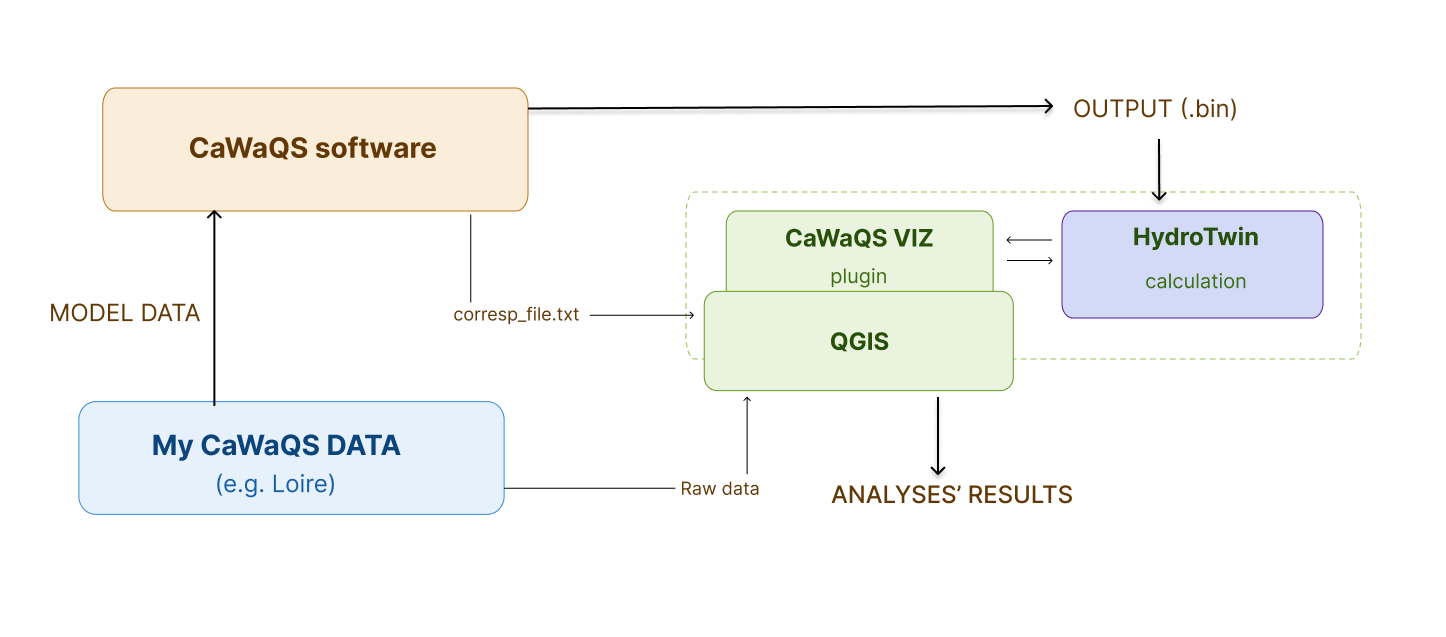
\includegraphics[width=0.9\linewidth]{4_application_scripts/fig/cvz_ecosystem.png}
    \caption{The \cwv~ecosystem --- position of the plug-in within the \cawaqs~toolchain.}
    \label{fig-cvz-ecosystem}
\end{figure}

\section{The Three Layers of the Backend}
\label{sec-layers}

HTAS is organised as a \textbf{three-level architecture} in which each level may call the level below it, never the level above. Each level has one canonical entry module, and imports point \textbf{strictly downward} (L1~$\rightarrow$~L2~$\rightarrow$~L3): never up, never sideways within a level. Because every dependency points downward, the layers can never form an import loop --- the dependency graph is acyclic.

\begin{lstlisting}[language=bash, caption={The three backend layers and their canonical entry modules.}, label={code-layers}]
L1 - HT CLIENT - MACRO        ht/client/hydrological_twin_client.py       (may import L2, L3)
L2 - HT DEVELOPER - MICRO     ht/developer/hydrological_twin_developer.py (may import L3)
L3 - SERVICES - ELEMENTARIES  services/                                   (imports nothing in ht/)
\end{lstlisting}

Taken together with the QGIS-side layers (frontend and interface), the roles are summarised in \cref{tab-layers}.

\renewcommand{\arraystretch}{1.3}
\begin{table}[H]
    \centering
    \begin{tabularx}{\linewidth}{>{\raggedright\arraybackslash}m{3.6cm}|X}
        \hline
        \textbf{Layer} & \textbf{Role} \\
        \hline
        \textbf{Frontend} \newline \script{frontend/} & QGIS dialog boxes. They own user interaction and route a single coarse call per workflow to the interface. \script{Qt}/\script{PyQt5} lives here and only here. \\
        \hline
        \textbf{Interface} \newline \script{interface/} & \script{ExploreData} is the \textbf{only} gateway to the backend; \script{GeoDataProvider} turns QGIS vector layers into \script{GeoDataFrame}s so the backend stays QGIS-agnostic. \\
        \hline
        \textbf{L1 - HT CLIENT - MACRO} \newline \script{ht/client/} & \script{HydrologicalTwinClient} exposes one method per user-facing dialog operation. Each delegates to a matching \script{operations\_client.run\_*} that owns the full \script{fetch}~$\rightarrow$~\script{transform}~$\rightarrow$~\script{render} chain and returns a typed \script{*Result} dataclass. Zero \script{qgis}/\script{PyQt5} imports --- usable from a notebook today, from an HTTP server tomorrow. \\
        \hline
        \textbf{L2 - HT DEVELOPER - MICRO} \newline \script{ht/developer/} & \script{HydrologicalTwin} is the micro-verb facade exposing 8 canonical verbs with an explicit \script{EMPTY}~$\rightarrow$~\script{CONFIGURED}~$\rightarrow$~\script{LOADED}~$\rightarrow$~\script{READY} state machine. Useful for notebook exploration and for operations not yet promoted to the client. \\
        \hline
        \textbf{L3 - SERVICES - ELEMENTARIES} \newline \script{services/} & Finest-grained computations and I/O: operators, renderer, twin-state reads and disk-cache provisioning (\script{twin\_io.py}), and leaf data DTOs (\script{io\_types.py}). No module under \script{services/} imports from \script{ht/} --- the import graph is a strictly downward, acyclic DAG. \\
        \hline
    \end{tabularx}
    \caption{Roles of the frontend, interface, and the three backend layers.}
    \label{tab-layers}
\end{table}

\script{ExploreData} calls \textbf{the client} for coarse operations (the normal path) and can still reach the developer twin \textit{via} \script{client.\_twin} for low-level micro-verb calls. A more annotated view of the data flow is given in \cref{fig-architecture-overview}.

\begin{landscape}
    \begin{figure*}
        \centering
        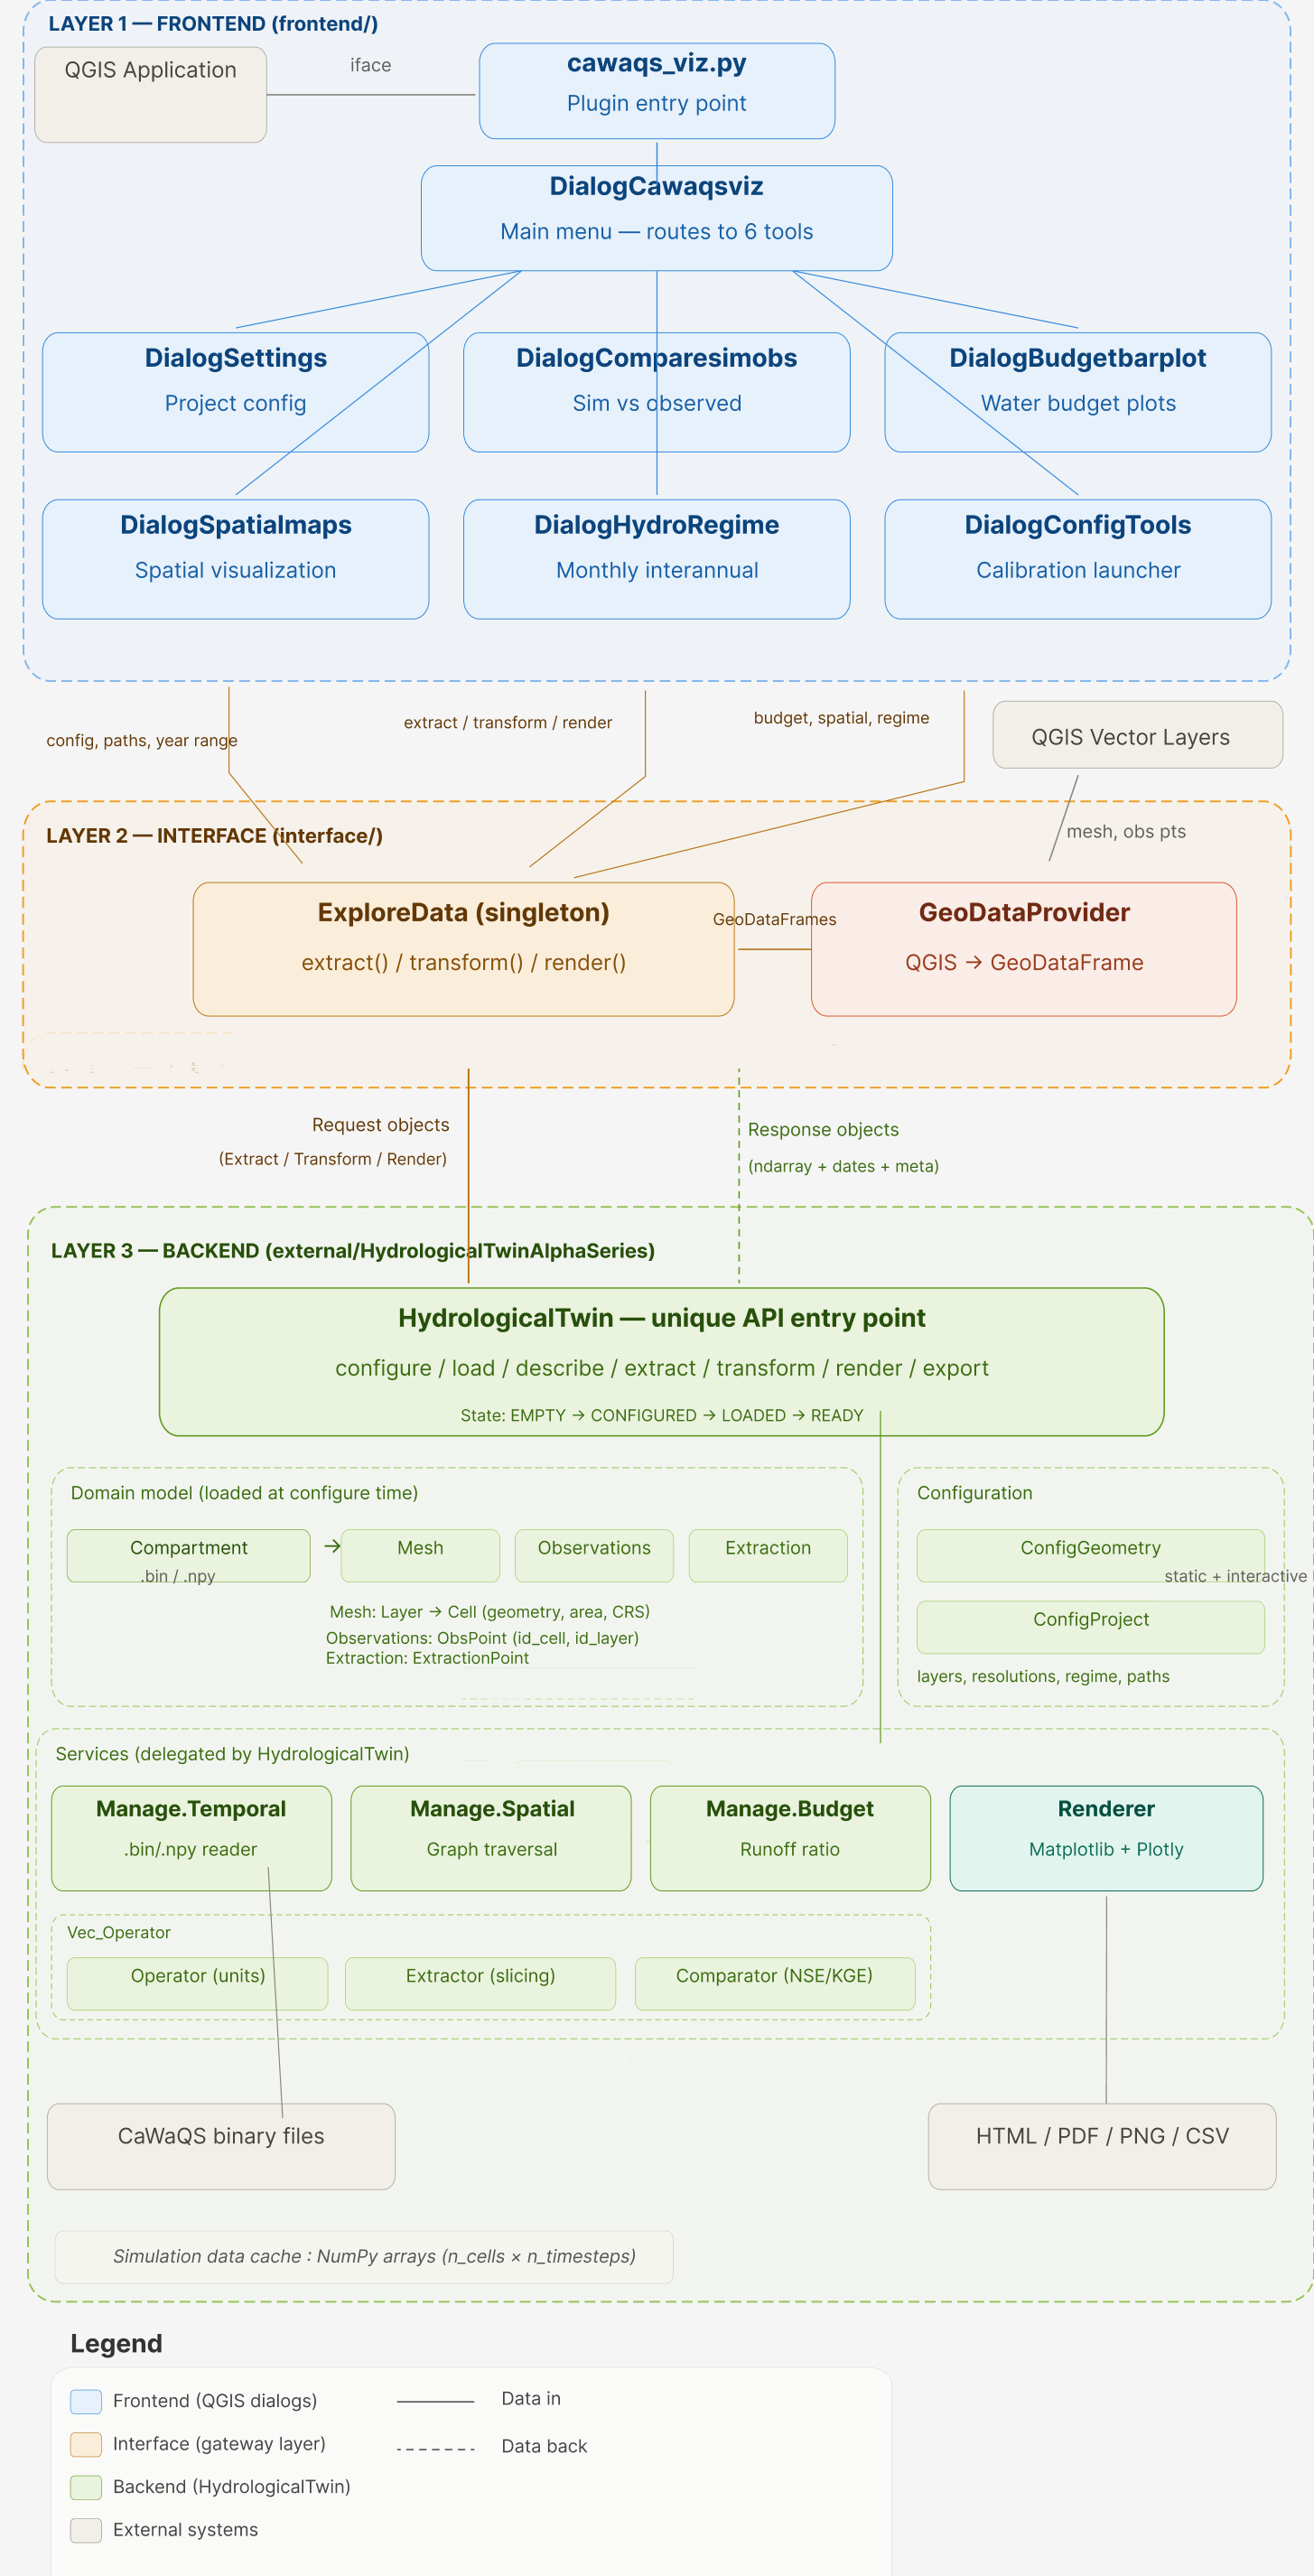
\includegraphics[width=1\linewidth]{4_application_scripts/fig/architecture_developer_overview.png}
        \caption{\cwv~+~HTAS architecture --- detailed component diagram with data flow.}
        \label{fig-architecture-overview}
    \end{figure*}
\end{landscape}

\section{Example Workflow: the Budget Bar Plot}
\label{sec-example-workflow}

The following walk-through shows what happens, step by step, when a user creates a water budget bar plot. It is one of the most complete workflows, chaining \script{fetch}~$\rightarrow$~\script{transform}~$\rightarrow$~\script{render}, and it is useful for understanding the number of round-trips between layers --- especially when designing the future server API.

\begin{enumerate}
    \item In the \script{DialogBudgetbarplot} dialog box, the user selects variables, a period, a frequency, and an aggregation.
    \item The dialog issues a \emph{single} coarse call to \script{ExploreData}, which forwards it to \script{HydrologicalTwinClient.budget\_barplot(**kwargs)}, which in turn calls \script{operations\_client.run\_budget\_barplot}.
    \item For each variable (rain, ETR, infiltration, runoff), the orchestration calls \script{twin.fetch} (reads the simulation matrix from disk through the services layer) then \script{twin.transform} (spatial mean + temporal aggregation).
    \item A final \script{twin.render} call produces the plot; the renderer writes a PNG and a CSV to disk and returns their paths.
    \item The paths are bundled into a \script{BudgetBarplotResult} dataclass and returned up the chain to the dialog, which opens the plot file.
\end{enumerate}

What this reveals for API design:

\begin{itemize}
    \item today, everything between \script{ExploreData} and the developer twin is \textbf{in-process}. The natural network seam is the \script{ExploreData}~$\rightarrow$~\script{Client} boundary, not \script{ExploreData}~$\rightarrow$~\script{HydrologicalTwin};
    \item \textbf{one coarse operation = one server round-trip}. The dialog calls \script{client.budget\_barplot(...)} once; the inner loop of 4 fetches + 4 transforms + 1 render stays server-side inside \script{run\_budget\_barplot}. The former ``9-calls-per-plot'' cost collapses to a single call at the network boundary;
    \item \textbf{the client \emph{is} the future HTTP surface.} Each \script{HydrologicalTwinClient} method maps cleanly to one endpoint, with a typed \script{*Result} dataclass as the response schema. The developer micro-verb API stays available for notebook-style exploration;
    \item \textbf{rendering still writes to disk.} When the client moves server-side, render outputs will need to return data (or signed URLs) instead of local file paths --- the \script{*Result} dataclasses are the right place to evolve that contract.
\end{itemize}

\section{Key Properties}
\label{sec-key-properties}

\begin{itemize}
    \item the \textbf{interface layer} is the cut point for a future server deployment --- everything below it could run remotely;
    \item the backend \textbf{never imports} QGIS or \script{Qt} (enforced by CI);
    \item all backend calls use \textbf{Request/Response objects} (e.g. \script{ExtractRequest}~$\rightarrow$~\script{ExtractValuesResponse});
    \item the \script{HydrologicalTwin} follows a \textbf{state machine} lifecycle: \script{EMPTY}~$\rightarrow$~\script{CONFIGURED}~$\rightarrow$~\script{LOADED}~$\rightarrow$~\script{READY}.
\end{itemize}
